
\chapter{Introduction}
\label{sec:intro}

%This is a general introduction to what the thesis is all about -- it is not just a description of the contents of each section. Briefly summarize the question (you will be stating the %question in detail later), some of the reasons why it is a worthwhile question, and perhaps give an overview of your main results. This is a birds-eye view of the answers to the main %questions answered in the thesis.

Procedural modeling is an exciting research area with trumendous potential for virtual worlds. Virtual worlds range from games, to simulations and virtual communities. These worlds are often very large and with advances in technology and user demand they rapidily grow larger for each new application. The problem is that space in these vast virtual worlds needs to be filled with interesting content. Creating such high amounts of content by hand does provide nice job opportunities, but if we could generate the same content with a set of parameters and the push of a button the choice is rather obvious. However, time and money efficiency are not the only arguments for the development of procedural methods. By studying real world objects or sets of real world objects in order to dynamically synthesise them in virtual worlds we gain a deeper knowledge of the characteristics of these objects and relationships between different objects. 

A couple of succesful existing procedural modeling implementations are interesting to discuss. In games, procedural methods have been employed for the generation of worlds with restricted sets of environmental elements, such as dungeons and mazes. A good example is the game "Diablo 2". The game "Spore" was one of the first games that heavily utilized procedural modeling techniques for a considerable part of content in the game. A very interesting project that is in development at the time of writing, is the game "Love" (figure \ref{fig:love}) developed by a single man. Procedural generation is used extensively for every part of this game.
      
\begin{figure}[htb]
\centering
\subfigure[World]{
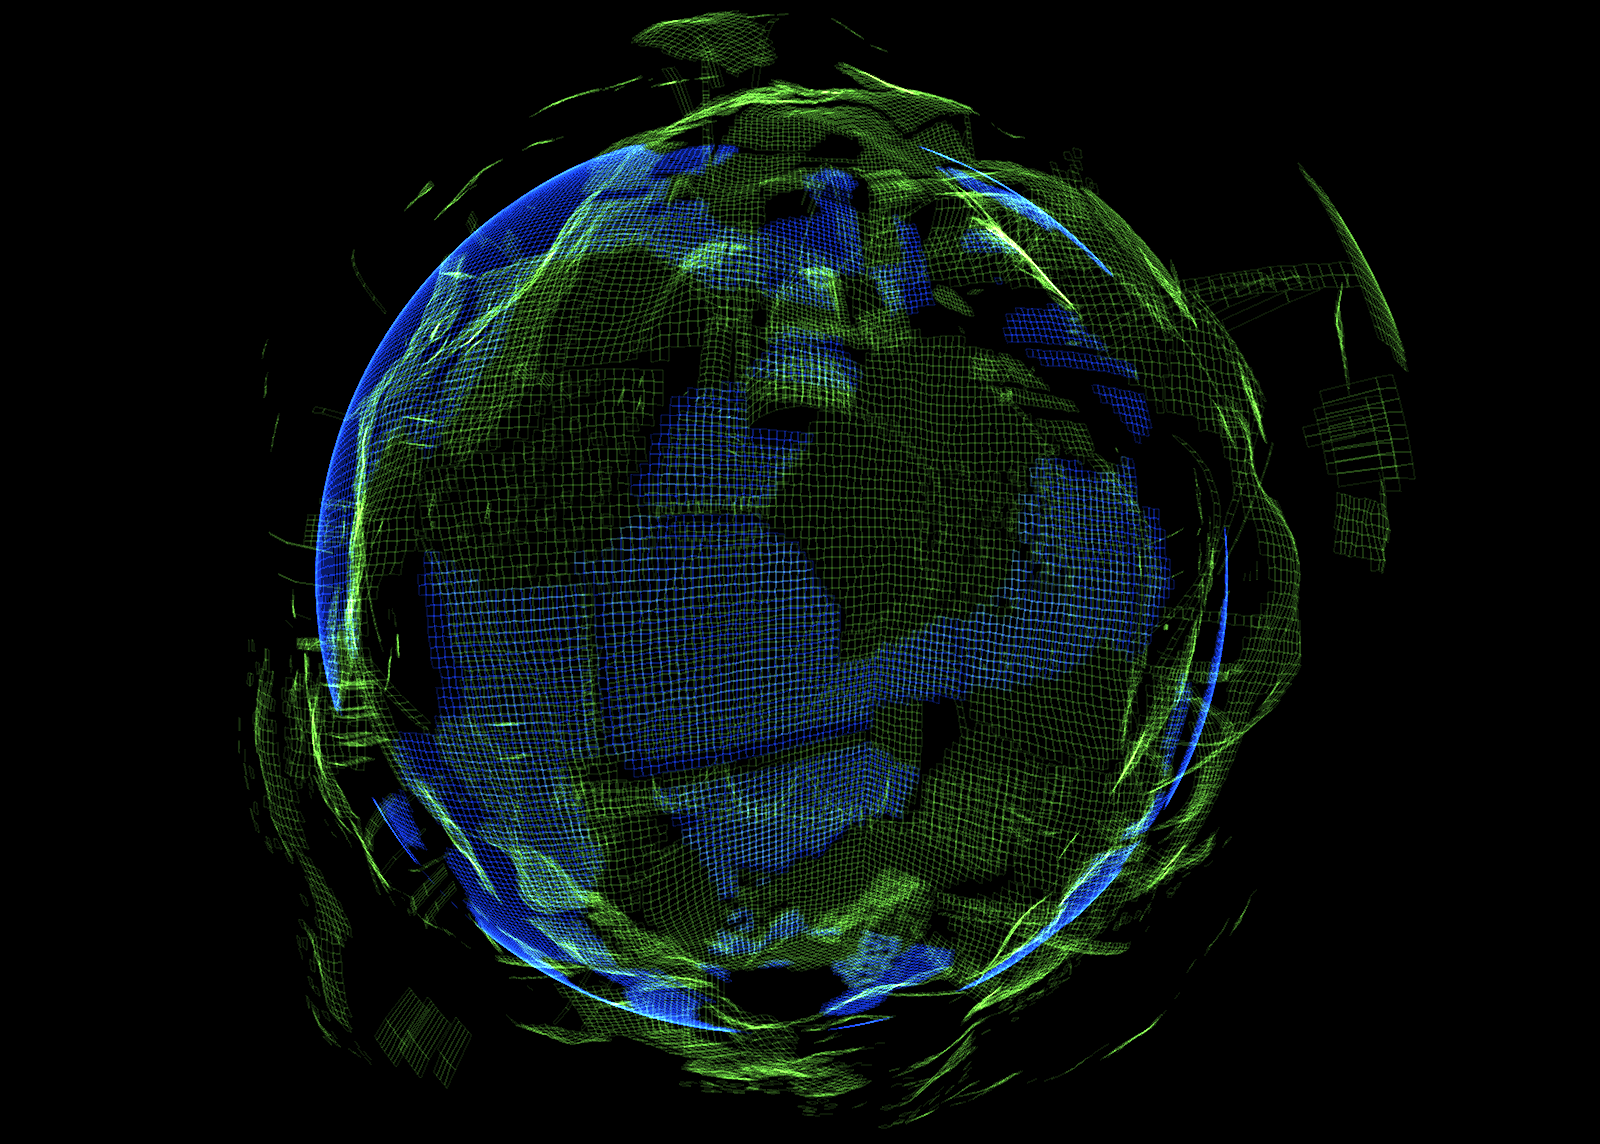
\includegraphics[width=100px]{images/love/world.png}
\label{fig:subfig1}
}

\subfigure[Ingame Environment]{
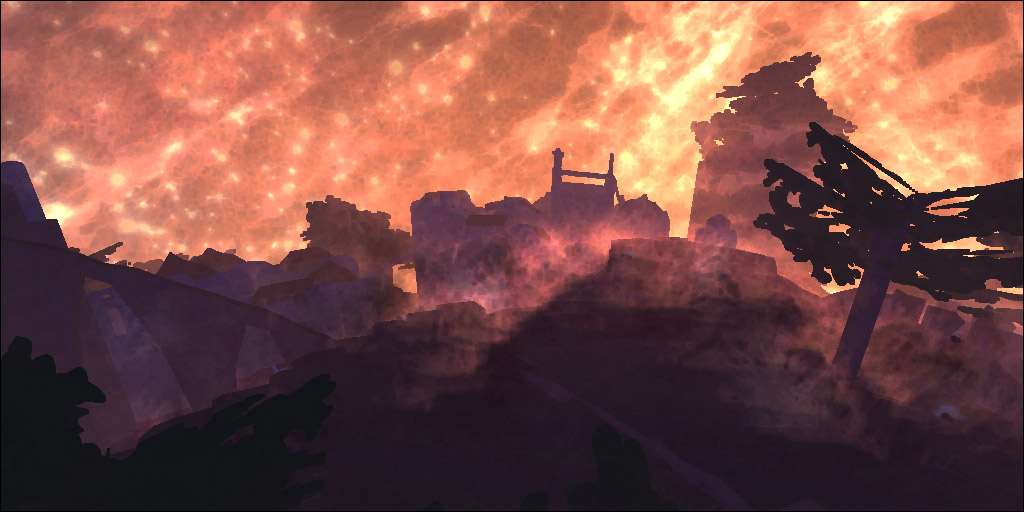
\includegraphics[width=100px]{images/love/love_city5.jpg}
\label{fig:subfig2}
}
\label{fig:love}
\caption[]{Screenshots of the game Love}
\end{figure}


This thesis adresses the problem of creating procedural architecture in the special case of restrictions and possibilities enforced by geometric properties of tree-like support-structures. A side goal for this research was to develop methods for intuitive interactive control for this specific procedural modeling method. 

%Regarding user control and procedural techniques it is important to strike a balance which allows for a fast %and intuitive building process, and meanwhile the user should have just the right amount of control to make the %scene to its liking.

%Rewriting systems, l-systems waarna shape grammars volgen
%The Shape grammar concept was originally coined by Stiny in his much cited \emph{"Shape and Shape Grammar"} \citep{Stiny80}.
%<hier de description van een shape>

Visual modeling of plant development is a field which started in 1962, when Ulam applied cellular automata to 
simulate the development of branching patterns \citep{PrzemyslawPlants}. A formalism for modeling plants was proposed by Lindenmayer 
in 1968, this formalism was called L-systems since. The following definition of an L-system is given by Przemyslaw \citep{PrzemyslawPlants}: 

\begin{quote}
An L-system is a parallel rewriting system operating on branching structures represented as bracketed strings of symbols with associated parameters, called modules. Matching pairs of square brackets enclose branches. Simulation begins with an  initial string called the axiom, and proceeds in a sequence of discrete deriviation steps. In each step, rewriting rules or productions replace all modules on the predeccesor string by succesor modules.   
\end{quote}   

Przemyslaw \citep{PrzemyslawPlants} has employed and extended the l-system formalism for realistic visualisation of entire plant ecosystems. Within a ecosystem organisms interact with each other and this interaction determines many properties for individual organisms; such as growth rate. Since the original L-system formalism does not account for communication between two processes, Przemyslaw proposed \emph{open l-systems} which incorporates \emph{communication modules}.    
  
L-systems also proved to be useful in the field of urban procedural generation \citep{Wonka03}. 
Muller showed that the L-system formalism could be succesfully used for the generation of road networks and in lesser extent building generation. 

%hier wat over building, generation, city generatoin, texture generation.
%shape grammars

Techniques for tree generation in this thesis are based on L-systems, however these techniques are simplified to a certain degree since the modeling of plants is not the maintopic of this thesis. We have used the l-system formalism to generate simple branching tree structures. We did not strive to generate visually realistic models of trees since this has already been achieved by many people before me with impressive results. Instead our simplified method generates the main structure of a tree which is then used as input in our method to generate configurations of architectural elements. 

%<hier resultaat van treehouse generatie module>

It is the case that traditional general purpose modeling software is very time consuming for the creation of complex scenes as a result of the lowlevel tools they feature. Special purpose modeling tools such as cityEngine \citep{Muller06} (in the case of urban modeling) and speedTree (in the case of modeling plants and trees) provide procedural methods to generate objects within a certain class with very high time effiency. However the human touch still remains a very important part of the modeling procedure. Eastatics are very hard to turn into a set of formal rules on which an algorithm can operate.

The special purpose modeling tool for the generation of organic geometry and treehouse architecture that was developed for this thesis provides the user with intuitive interaction tools to allow easy manipulation.        


%\old{   
%The research which preceded this document strived to construct an intuitive organic modelling method for the creation of 2D maps. The central focus of this research has been on methods %for construction of dynamic structures using real-time growth models. To enable a large degree of control over these dynamic structures the is a need for skeletons. A large part of this %thesis is about constructing skeleton representations for dynamic structures. There obviously is a realtime demand in order to enable realtime interactivity, which means building such %skeletons should above all be an efficient process.    
%}

\section{Overview}
\label{subsec:overview}

This thesis is structured as follows. In the next section I will discuss related work. In the related work section I will bring my thesis into context with regard to procedural modeling of trees, architecture and generation of levelmaps. A precise statement of the problem and why it's an interesting problem to solve will follow in section \ref{sec:problem}. 

In section \ref{sec:concept} I will present the conceptual system model. The method for the generation of the forest layout and the generation of the tree geometry is presented in section \ref{sec:pfg}.  
 
With the forest geometry in place we are ready to review the planning method which is responsible for the construction of a connected graph representing a tree community. I will conclude the method description with a look at the final stage of the pipeline, translating the symbols from the nodes and edges of the graph to the geometrical architectural elements. Section \ref{sec:UIT} discusses user interactivity and usability of the proposed system. The last two sections present results and conclusions respectively.     
